%===================================== CHAP 4 =================================

\chapter{Four Point Probe}

    %intro to resistivity 
    
    The four-probe technique is a method that allows for sensitive resistivity measurements by eliminating the resistance of the measurement probes and contacts from a measurement. In a two point resistivity measurement the resistance is the sum of the resistance of the leads, the resistance of the contacts and the resistance of the sample. %[current spreading etc, semicondutor devices]
    When the resistance of the leads and contacts becomes comparable to the sample resistance the method is no longer useful for accurately determining the resistance. The four-probe methods uses four contacts to the sample; two probes supply current to the sample and the voltage is measured across the remaining two probes. In the ideal case, due to their high impedance, no current flows through the voltage probes eliminating any contribution to the resistance due to the contacts and leads. Typical four-probes are designed to measure semiconductor wafers and thin films and consist of four co-linear Tungsten probes with constant spacing. While other geometries are possible %[citations]
    we will now consider this geometry for the rest of the text, unless otherwise specified. 
    
 \section{Sample Geometry}
 
    For isotropic materials, electrical resistivity is a property that relates the current density in a sample to the electrical field applied to it. This gives the relation \begin{equation}
        \rho = \frac{E}{J}
    \end{equation}
    Experimentally it is the Resistance $R$ that is measured, which only defines a relationship between the current $I$ and the Voltage $V$ giving the familiar expression: \begin{equation}
        R = \frac{V}{I}
    \end{equation}
    
    In order to determine the resistivity of the sample, the geometry of the sample, and size and placement of the contacts must be known as these define the current paths within the sample. There are many papers that 
    
    
    For the case of the co-linear four point probe and a homogeneous sample, we can define the resistivity $\rho$ as:
    
    \begin{equation}
    \rho = G * \frac{V_{2-3}}{I_{1-4}}
    \end{equation}
    where G is a correction factor that depends on the geometry of the sample and, the position of the contacts and their spacing. Where the subscript denotes the probe numbers, e.g. $V_{2-3}$ refers to the voltage between probes 2 and 3. For special cases the correction factor can be easily calculated. 
    %Semi infinite volume
    \begin{equation}
        \rho = 2 \pi s * \frac{V}{I} 
    \end{equation}
    where s is the probe spacing.
    %Thick Sample 
    \begin{equation}
        \rho = 2 \pi s *T_1 (\frac{t}{s})* \frac {V}{I} 
    \end{equation}
    
    
    %Thin Sample
    \begin{equation}
        \rho = \frac{\pi}{\ln{2}} * t *T_2 (\frac{t}{s}) * \frac{V}{I}
    \end{equation}
    where t is the thickness and $T_2 (\frac{t}{s})$ is a correction factor for when $(\frac{t}{s})$ is not much less than 1. For t = s the correction factor is $7.16 \%$
    
    
    %correction for semicircular shape
    %correction for 
\section{Finite Size Contacts}
 The previous four point probe equations are derived for measurements made with ideal point like contacts and a high impedance voltmeter so that no current can flow through the contacts. In any real situation there will be a finite area of contact between the probe and the sample and finite interface resistance between the contacts and sample. This will allow current to flow into the contacts and will disturb the potential and current distributions in the sample \cite{Zimney2007CorrectionStudy}. With lithographically defined micro scale contacts this contact area may become large compared to the probe spacing, and the effects of the metal contacts must be considered. %here? 
 Two situations in this work required the use of small contact spacing. First is the occurrence of cracks with the fiber which limited the continuous length of fiber, and second is high resistivity fiber cores which require a small contact spacing in order to drive a measurable current through the sample without exceeding the voltage source range of the source meter unit. 
 
  
\begin{figure}[h]
  \centering
    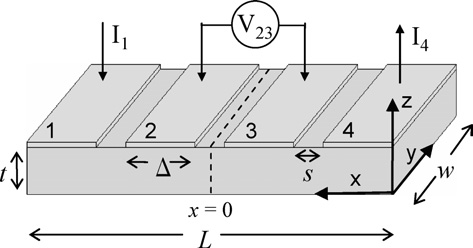
\includegraphics[width=0.5\textwidth]{fig/4pp/finite_size_contacts.png}
 \caption{Schematic of the co-linear 4-probe configuration with electrodes that span the width of the specimen. Figure and caption reprinted from \cite{Zimney2007CorrectionStudy}.}
\label{fig1}
\end{figure}
 
   
 
 Several theoretical and experimental studies have been done on the influence of finite size contacts for co-linear resistivity measurement \cite{Zimney2007CorrectionStudy}, \cite{Mak1989SpecificArsenide}, \cite{Ilse2014GeometricalMeasurements}. Zimney et al. and Mak et al. focus on rectangular contact bars and are most relevant for this analyses. Zimney et al has used finite element studies to investigate the influence of rectangular contacts spanning the width of a sample as shown in figure \ref{fig1}. These results may be applied to this work under the approximation that the semicircular fiber core cross section is rectangular. In this paper it is assumed that the resistivity of the contacts is much lower than the sample (the contacts are equipotential), the sample is homogeneous and that the interface resistivity is ohmic.  %talk about what defines interface resistivity. ohmic nonohmic elements. 
 \begin{table}[b]
\begin{center}
    \begin{tabular}{|l|l|l|  }
    \hline
  %  \textbf{No.} & \textbf{Data 1} & \textbf{Data 2} \\ \hline
     The thickness ratio & $TR = \frac{t}{s}$ \\ 
     The electrode ratio & $ER =  \frac{\Delta}{s}$ \\ 
     The interface resistance factor & $\alpha = \frac{R_c}{R_m}$ \\
     \hline
    \end{tabular}
\end{center}
\caption{Dimensionless variables used in the analysis of Zimney et al. simplified for the case of an isotropic material \cite{Zimney2007CorrectionStudy}}
\label{Tab1}
\end{table}
 
As the contacts span the sample width there is no current flow in the y direction \ref{fig1} and the analysis is equivalent to the two dimensional system. Several dimensionless variables describe the the geometry and are found in Table \ref{Tab1}. The contact spacing $s$ is defined as the distance between the inner edges of the voltage sensing contacts. $R_m$ is the measured 4 terminal resistivity, $R_c$ is the interface resistance and $\Delta$ is the contact width. 

For the given geometry the resistivity is given by the following relation: \begin{equation}
    \rho   = F \frac{wt}{s}R_m = F \frac{wt}{s}\frac{V_m}{I_m}
\end{equation} where F is a correction factor accounting for any perturbation in the current distribution due to the influence of sample thickness and presence of contacts, and the subscript m signifies a measured value. Due to the definition of s is the distance between inner edges of the contact pads, F will not be equal to 1 for the case of a uniform current distribution. This is because the measured voltage will not be the voltage at the edge of the contact, e.g for $ER = 1$, $F = .5$.


 
 \begin{figure}[]
  \centering
    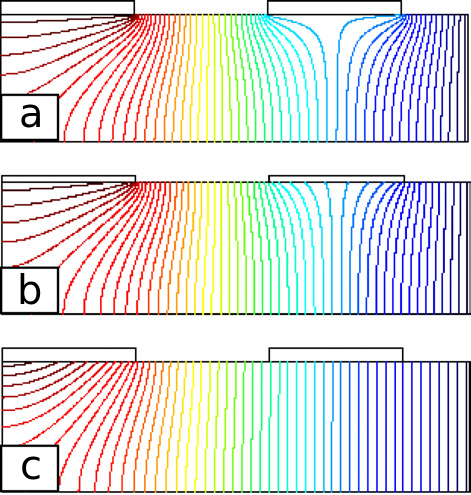
\includegraphics[width=0.5\textwidth]{fig/4pp/finite_contact_contour.png}
 \caption{ Potential contour plots for varying interface resistivity with $ER=1$ and $TR= 1$. The interface resistance increases from top to bottom: (a) \hspace{.5mm} $\alpha=0$, (b) \hspace{.5mm} $\alpha=0.1$ and (c) \hspace{.5mm} $\alpha>> 1$ . Figure and caption adapted from \cite{Zimney2007CorrectionStudy}.}
 \label{fig2}
\end{figure}


Figure \ref{fig2} illustrates the change in potential for varying contact resistivity for the case of $ER$ and $TR$ equal to one. The left electrode is the current source, and the right electrode is the voltage sensing electrode. 

The influence of the contacts can be easily understood under two extremes of infinite or zero specific contact resistivity. With zero specific contact resistivity current will easily flow into the low resistivity contact pads, and the contact essentially short circuits the sample beneath. No potential drop occurs under the contact pad. With high specific contact resistivity, no current will flow through the contact, and the contact is isolated from the sample leaving the potential in the sample beneath unchanged \ref{fig1}(c). For intermediate values of contact resistivity a portion of the current will flow through the contact causing a potential drop across the contact-sample interface.
With these considerations it is shown that it is non-trivial  to determine the contact spacing that corresponds to the position in the sample of the measured potential. In the first case the potential in the contacts will be an average of the potential beneath the contacts \cite{Zimney2007CorrectionStudy} %more here?
and the the spacing is measured from the center of the contact, and the second case the measured potential is that of the sample at the edge of the contact, and the spacing is measured from the edge.


%what is important: order of magnitude of contact resistivity. How the correction factor changes. h
%$L = 3s + 4\Delta$

Figure \ref{ER1} a plots F against TR for the limiting cases of high and low contact resistivity ($\alpha = 0$ and $\alpha >> 1$ and with $ER = 1$ . This shows that the thickness of the 


\begin{figure}[htb]
  \centering
    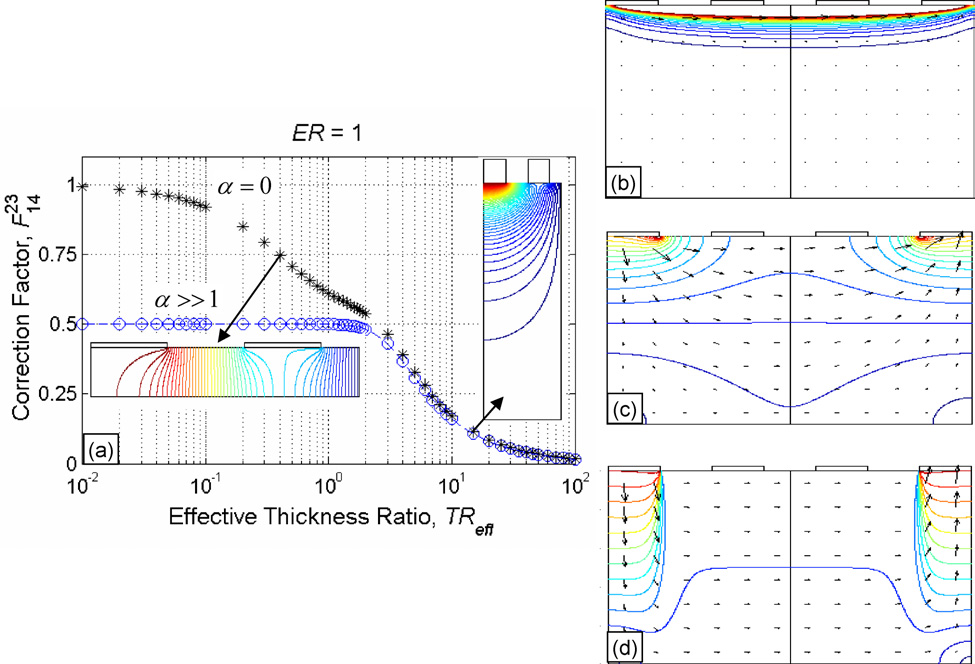
\includegraphics[width=\textwidth]{fig/4pp/ER1.png}
 \caption{  Figure and caption adapted from \cite{Zimney2007CorrectionStudy}.}
 \label{ER1}
\end{figure}


\cleardoublepage
